\chapter{De-Entanglement of Content - Case study with Acoustic Unit Discovery}

\section{Problem Introduction}
A major bottleneck in the progress of many data-intensive language processing tasks such as speech recognition and synthesis is scalability to new languages and domains. 
Building such technologies for unwritten or under-resourced languages is often not feasible due to lack of annotated data or other expensive resources. 
A fundamental resource required to build such a stack is a phonetic lexicon - something that translates acoustic input to textual representation. Having such a lexicon, even if noisy, can help bootstrap speech recognition models, synthesis, and other technologies. Typical approaches may involve a pivot language or bootstrapping or adapting from a closely related high-resource language.
But, this can be a deceptively non-trivial task due to linguistic differences which can pose inherent difficulties. 
For instance, it may be unreasonable to analyze a Sino-Tibetan language using English as a source. Moreover, using an additional language might make the model learn unintended surface level associations or biases between the participating languages that prevent them from generalizing across languages. Associations between these languages over a set of units that may better generalize to other languages. Therefore, in this paper we are interested in discovering the appropriate acoustic phonetic units. 

\begin{figure}[t]
\centering
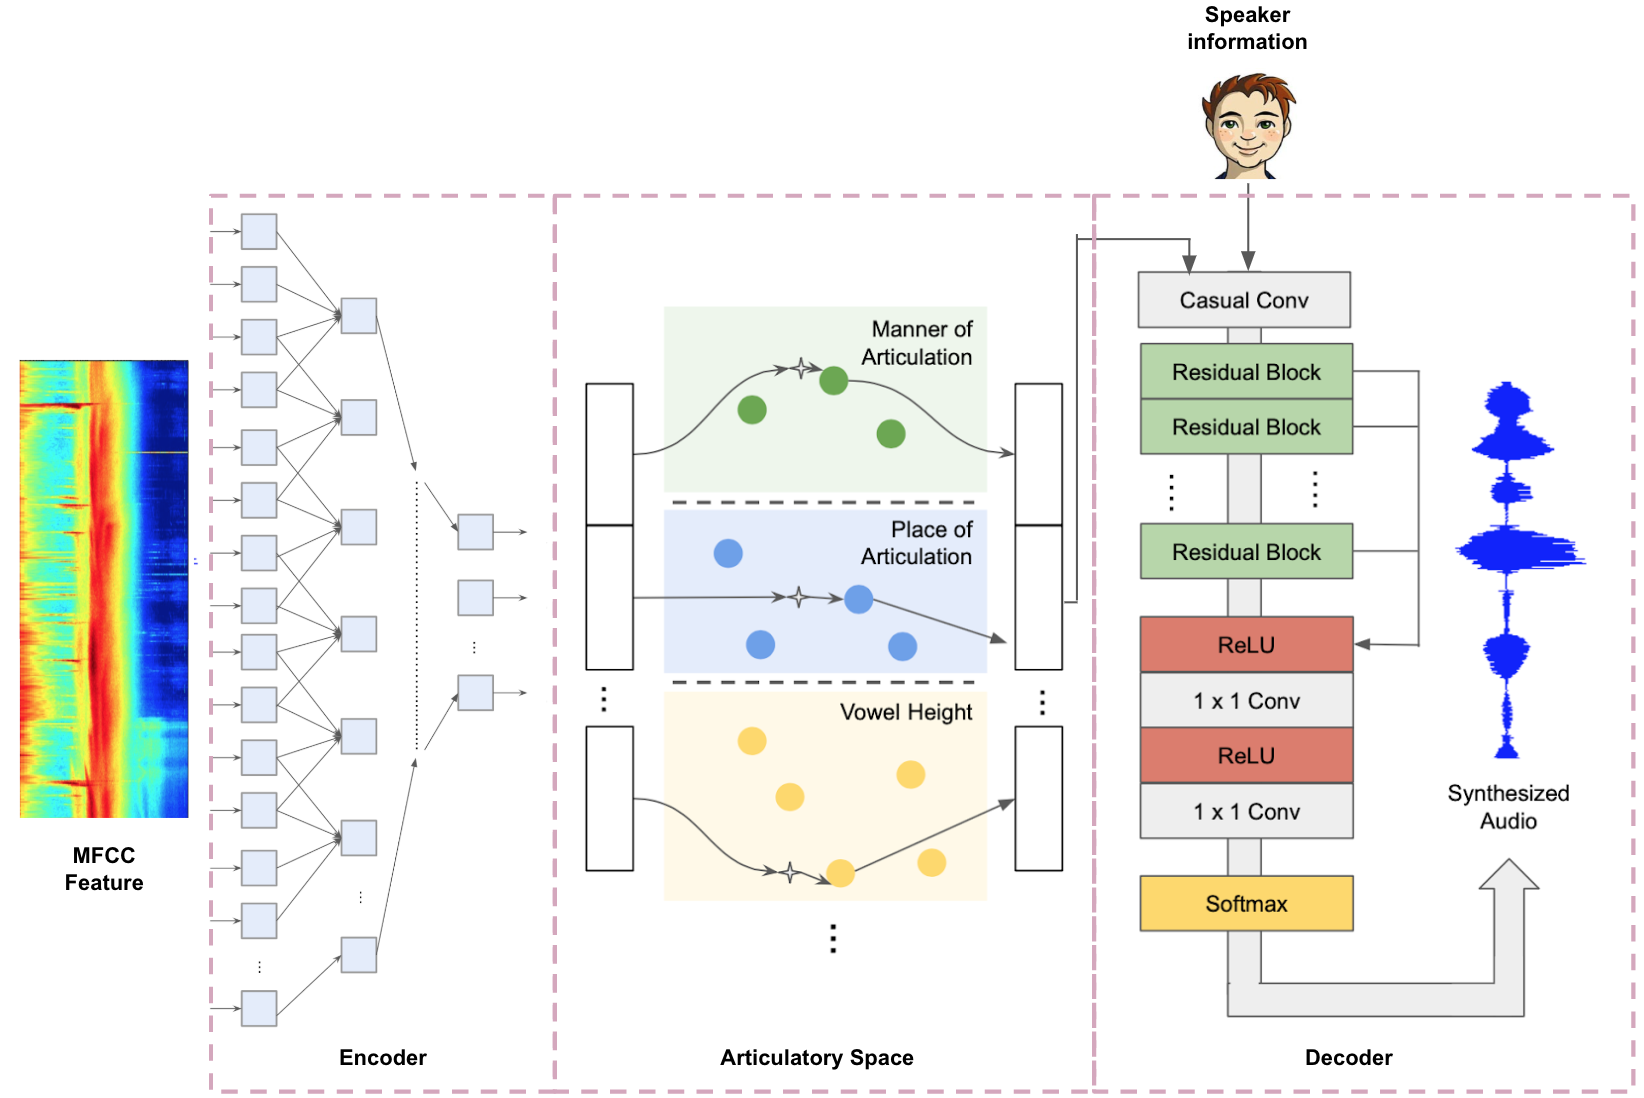
\includegraphics[width=80mm,scale=0.5]{images/vaconda_architecture_zerospeech2019.png}
\caption{Illustration of our procedure for automatically discovering acoustic units from a speech utterance. We pass the speech utterance through a downsampling encoder. The encoded representation is hashed to a latent code based on a discrete articulatory prior bank. The code is passed to the decoder, a WaveNet using speaker embeddings as global conditioning that regenerates audio. } 
\label{frame_replacement_overview}
\end{figure}  


In ZeroSpeech Challenge\citep{zerospeech2019} resynthesis is considered a good proxy task to evaluate the performance of systems when training using unsupervised approaches. To accomplish this we use neural generative models. %Resynthesis might be a good proxy. 
Deep Neural Generative models have seen a tremendous amount of progress in the recent past. These models aim to model the joint probability of the data distribution and the conditioning information as a product of conditional distributions. Typical implementations of such models follow an autoregressive framework, although other formulations have been suggested as well. Such models have been shown very effective in addressing one of the major challenges with conventional vocoding techniques - fidelity. 
Neural generative models has been shown to generate speech that rivals natural speech when conditioned on predicted mel spectrum \citep{shen2017natural}. Speech has a lot of natural variations in terms of content, speaker, channel information, speaking style, prosodic variations, etc. Accordingly, we are interested in models which have flexibility to  marginalize such variations but preserve the phonetic content and distinguish meaningful differences between phonetic units.To accomplish this, we employ sequence to sequence models with latent random variables (referred to as latent stochastic models hereafter). These models provide a mechanism to jointly train both the latent representations as well as the downstream inference network. They are expected to both discover and disentangle causal factors of variation present in the distribution of original data, so as to generalize at inference time. While training latent stochastic models, optimizing the exact log likelihood can be intractable. To address this, a recognition network is employed to approximate the posterior probability using reparameterization \citep{vae}. When deployed in encoder-decoder models, this approach is often subject to an optimization challenge referred to as KL-collapse \citep{bowman_continuous}, wherein the generator (usually an RNN) marginalizes the learnt latent representation. Typical approaches to dealing this issue involve annealing the KL divergence loss~\citep{bowman_continuous,zhou2017multi}, weakening the generator \citep{zhao2017learning} and ensuring the recall using bag of words loss.  In our work, we present an approach to deal with the KL-collapse problem by vector quantization in the latent space.  Building on \citep{vq-vae, chorowski2019unsupervised}, we add additional constraints in the prior space forcing the latent representations to follow articulatory dimensions: The encoded representation is hashed to a latent code based on a articulatory prior bank designed using a discrete codebook. Our decoder is a conditional WaveNet using speaker embedding as global embedding trained to regenerate input audio using the  code sequence as local information. 


\section{Background - Acoustic Unit Discovery}

Let us consider a speech corpus X which consists of speakers $\{ s_1, s_2...,s_n \}$. The goal of acoustic unit discovery is to come up with a set of units \textbf{U} that represent a speech utterance \textit{x} $\subset$ X allowing robust resynthesis. %comprehensively. 
The elements of such a set also might conform to desirable characteristics  such as being injective, consistent and compact, i.e. that different inputs should have discriminant acoustic units, but expected variance such as speaker or dialect should produce the same acoustic units. %, and the set of units should be 
% We aim to discover a minimal set of units to fit these goals.
%must be well corresponding to the acoustic vectors(predictable)


There have been numerous attempts to discover such acoustic units in an unsupervised fashion. In \citep{subword_diarization}, authors presented an approach to modify the speaker diarization system to detect speaker-dependent acoustic units. \citep{unsupervised_AMtraining_ArenJansen} proposed a GMM-based approach to discover speaker-independent subword units. However, their system requires a separate Spoken Term Detector. Recently, due to the surge of deep generative model, using unsupervised method such as auto-encoder and variational auto-encoder (VAE). \citep{badino_autoencoder} designed a stacked AutoEncoder using backpropagation and then cluster the representations at the bottleneck layer. To avoid quick transitions leading to repeated units, they employed a smoothing function based on transition probabilities of the individual states. \citep{hmm-vae_bhiksha} extended the structured VAE to incorporate the Hidden Markov Models as latent model. \citep{vq-vae, chorowski2019unsupervised} proposed VQ-VAE and argue that by vector quantization the ``“posterior collapse" problem could be circumvented.


\section{\textit{VACONDA}}
\label{proposed_approach}


\subsection{Analysis of optimization and de-entanglement}
\label{analysis}

WaveNet \citep{van2016WaveNet} is an autoregressive neural model with a stack of 1D convolutional layers that is capable of directly generating audio signal. It has been shown to produce generated speech that rivals natural speech when conditioned on predicted mel spectrum \citep{shen2017natural}. The input to WaveNet is subjected to corresponding gated activations while passing through each dilated convolutional layer and is classified by the final softmax layer into a $\mu$ law encoding.  The concrete form of the residual gated activation function is given by following equation:


\begin{equation} \label{WaveNet_Eqn}
\begin{split}
  r_d(x) = tanh(W_{f} * x) \odot \sigma (W_{g} * x)  \\ 
\end{split}
\end{equation}

\noindent where $x$ and $r_d(x)$ are the input and output with dilation $d$, respectively. The symbol $*$ is a convolution operator with dilation $d$ and the symbol $\odot$ is an element-wise product operator. $W$ represents a convolution weight. The subscripts $f$ and $g$ represent a filter and a gate, respectively. The joint probability of a waveform \textbf{X} can be written as:


\begin{equation} \label{WaveNet_gen_Eqn}
\begin{split}
  P(X | \theta)  = \prod_{t=1}^{T} P(x_t | x_1, x_2 .. x_{t-1}, \theta)  \\
\end{split}
\end{equation} 

\noindent given model parameters $\theta$. During implementation of WaveNet, the autoregressive process is realized by a stack of dilated convolutions. The final output $y_t$ at time step $t$ can be expressed mathematically as:

\begin{equation} 
\begin{split}
  \hat{y_t} \sim \sum_{d=0}^{D} h_d * r_d(x) \\
\end{split}
\label{WaveNet_Eqn}
\end{equation} 

\noindent where $x$, $y$ represent input and output vectors; $D$ is the number of different dilation used and $d$ is the dilation factor; $h_d$ is the convolution weights. This stack of convolutions is repeated multiple times in the original WaveNet. Optimization in WaveNet is performed based on the error between predicted sample and the ground truth sample conditioned on previous samples in the receptive field alongside the local conditioning. Expressing the loss function being optimized mathematically the error at sample $t$ is:


\begin{equation} \label{discrete_Eqn}
\begin{split}
  l_t = Div(\hat{y_t} || y_t)
\end{split}
\end{equation} 

Here, we define the divergence similar to the \citep{salimans2017pixelcnn++}, To optimize this loss, the contribution from the individual convolution layers towards this global error function must be nullified. Now let us consider the expression for intermediate output for a single filter in Eqn~\ref{WaveNet_Eqn}:

\begin{equation}
\begin{split}
  x_{out}(t) = \sum_{\tau=0}^{t} h(\tau)x(t-\tau)
\end{split}
\end{equation} 

\noindent where $\tau$ is the receptive field covered by the model and $h(\tau)$ represents the discrete state representation at time $t$. Without loss of generality and dropping the term $\tau$ for brevity, the spectral representation generated by the model can be expressed as:

\begin{equation} \label{transfer_function_representation}
  Y(z)  = H(z) X(z) 
\end{equation} 


Considering the discrete nature of input from Eqn \ref{discrete_Eqn}, an interpretation of Eqn \ref{transfer_function_representation} is that the neural autoregressive model acts as the transfer function and is discretized by convolving with the samples from original signal. It has to be noted that this is similar to the formulation of source filter model of speech, specifically the periodic components aka voiced sounds. Voiced sounds typically represented as impulse train are convolved with the transfer function to generate spectral envelope. As a corollary, from Eqn \ref{discrete_Eqn} and \ref{transfer_function_representation}, we posit that the optimization in WaveNet model is performed by minimizing the divergence between true and approximate spectral envelope. Note that latent stochastic models such as VAEs are aimed to minimize the divergence between true and approximate posterior distributions of input data. The advantage with such models is the presence of stochastic random variables that capture the causal factors of variation in input based on some prior information about the distributional characteristics of data. Techniques aimed at this \citep{beta_vae} have shown that it is possible to effectively disentangle the factors of variation using stochastic variables. Hence, we postulate that it should be possible to augment WaveNet decoder with a suitable encoder and an appropriate prior distribution to disentangle the acoustic phonetic units from a given utterance. 


However, this is a deceptively non-trivial task. If the prior is too simplistic, such as unit normal distribution, the model is trivially incentivized to force the posterior distribution to closely follow the Gaussian prior distribution \citep{lossy_vae}, particularly early in training. This results in the decoder marginalizing out the latent variable completely, manifesting in poor reconstruction ability. On the other hand, making the prior distribution arbitrarily complex also leads to unreasonable constraints on the decoder. For instance, in scenarios that have categorical distributions as their output (tasks such as language modeling, machine translation, and image captioning among others) it is unintuitive to assume that the true prior that generates latent distribution is a Gaussian when the likelihood is based on discrete sequential data. We make an observation that dealing with speech presents a characteristic advantage - speech has both continuous as well as discrete priors. The generative process of speech assumes a Gaussian prior distribution which is continuous in nature. However, the language which is also present in the utterance can be approximated to be sampled from a discrete prior distribution. Exact manifestation of this in the linguistics can be at different levels: phonemes, words, syllables, subword units, etc. From the analysis presented in the previous section, we hypothesize that if we use background knowledge about the data distribution while designing the priors, we can help the encoder effectively disentangle the latent causal factors of variation in the data. In other words, this presents us with an opportunity to control what gets disentangled in the latent space by appropriately choosing a prior distribution. Therefore, we engineer our prior space to account for the phonetic information in the utterance by representing the prior as a discrete latent variable bank, similar to the filterbanks used for feature extraction from speech. Each discrete latent variable has a different set of states reflecting one of the articulatory dimensions. The specific design of our latent space is highlighted in Table \ref{articulatory features}.


\renewcommand{\arraystretch}{1.0}
\begin{table}[t]
\caption{Articulatory Features\label{tab:arti}}
\centering
\begin{tabular}{l | c | c}\toprule[\heavyrulewidth] \textbf{Feature name} & \textbf{Value} & \textbf{Details} \\
\toprule[\heavyrulewidth]
vc & + - 0 & vowel or consonant \\
vlng & s l d a 0 & vowel length\\
vheight & 1 2 3 0 - & vowel height \\
vfront & 1 2 3 0 - & vowel frontness\\
vrnd & + - 0 & lip rounding\\
ctype & s f a n l r 0 & consonant type \\
cplace & l a p b d v g 0 & place of articulation \\
cvox & + - 0 & consonant voicing\\
asp & + - 0 & consonant voicing\\
nuk & + - 0 & consonant voicing\\
\bottomrule[\heavyrulewidth]
\end{tabular}
\label{articulatory features}
\end{table}



\section{Experiments}
\label{expts}


\subsection{ZeroSpeech 2019 dataset}
% The goal of ZeroSpeech dataset is to learn the Phonetic representation of the audio without any supervision, discover the symbolic representation of the audio, and resynthesize the audio using these unit. The evaluation metric look at both the quality of sub-unit and the resynthesized audio.

ZeroSpeech Challenge 2019: TTS without T is to propose to build a speech synthesizer without any text or phonetic labels~\citep{sakti2008development1, sakti2008development2, zerospeech2019}. The systems are required to extract the symbolic representation of the raw audio, and then re-synthesize the audio using these discovered units. There are three datasets in total: (1) \textit{Unit Discovery Dataset} provides audio from a variety of speakers and is used to unsupervised acoustic modeling, (2)  \textit{Voice Dataset} provides audio from the targeted speaker and is used for synthesizer modeling and (3)  \textit{Parallel Dataset} is intended for finetuning both the sub-systems. We have not utilized the parallel dataset for our observations in this study. The development language is English and the test language is Standard Indonesian. The system is constrained to not use any pre-existing resource or models. To ensure that the model generalizes out of the box, the hyperparameter will be fine-tuned only on the development dataset, and the model will be trained in test language under the same parameters. 

\iffalse
\begin{enumerate}
    \item \textit{Unit Discovery Dataset} provides audio from a variety of speakers and is used to unsupervised acoustic modeling
    \item \textit{Voice Dataset} provides audio from the targeted speaker and is used for synthesizer modeling
    \item \textbit{Parallel Dataset} is used for finetuning the both sub-systems
\end{enumerate}

The development language is English and the test language is Standard Indonesian. The system is refrained from using any pre-existing resource or models. To ensure that the model generalizes out of the box, the hyper-parameter will be fine-tuned only on the development dataset, and the model will be trained in test language under the same parameters. 
\fi

% \subsubsection{CSTR VCTK Corpus}

% CSTR VCTK is an English speech dataset, which contains 109 native speakers with various accents. Each speaker is required to record 400 sentences from newspaper, plus Rainbow Passage and an elicitation paragraph intended to identify the speaker's accent.

%\subsection{Implementation Details}

% CSTR VCTK Corpus includes speech data uttered by 109 native speakers of English with various accents. Each speaker reads out about 400 sentences, most of which were selected from a newspaper plus the Rainbow Passage and an elicitation paragraph intended to identify the speaker's accent
% 
% newspaper sentences,

\iffalse
Our voice building process employs the phone sharing approach as outlined in \citep{rallabandi_mixedlingual_IS2017} - where the combined phoneset is formed by the union of phones from both the languages - to build acoustic models. In this section, we present our approaches to generate the required bilingual acoustic data using just monolingual recordings. Specifically, in each of the subsections, we introduce the approaches we follow to artificially generate spectral content in English. We then follow the outlined procedure to build a bilingual voice using the native (L1) recordings and `pseudo English' (L2) recordings. 

In this section, present our approaches for ZeroSpeech 2019. Specifically, our aim is to build robust models capable of accomplishing (1) Discovering acoustic units given a speech utterance. and (2) Generating novel utterances conditioned on the discovered acoustic units. For this, we have built two systems: (1) System A which is a pipeline based approach and (2) System B which is an end-to-end approach. 
\fi 

\section{Baseline System}

We have a three-stage pipeline: (1) \textit{Unit Discovery}: We hypothesize acoustic units given a speech utterance using latent Stochastic Models; (2) \textit{Unit Alignment}: We fine-tune the alignment between the utterance and the proposed acoustic units ; (3) \textit{Unit Synthesis}: We build a speech synthesizer using the acoustic units and the target voice.


%In this section, we will elaborate on each of the three stages.

%\subsubsection{Acoustic Unit Discovery}
%\subsubsection{Acoustic Unit Alignment}

As proposed in \citep{sitaram2013bootstrapping}, we take the initially discovered transcription of the acoustic units for our speech corpus and train an ASR model on it. Then we re-encode the corpus using the ASR model, and train a TTS system on it. Here we using Bi-LSTM with CTC loss as our ASR model, and tacotron \citep{tacotron_transferlearning2multispeaker} as TTS system. 

% At each iteration, an acoustic model is trained from the parallel speech-transcription data. This acoustic model is then used to re-decode the speech data, and so on for 10 iterations. At the end of each iteration, we have produced a rebuilt acoustic model and a re-decoded transcript. These two are used to build a synthetic CLUSTERGEN \citep{black2006clustergen} voice (given the noise in the generated data, statistical parametric synthesis is appropriate) using Festvox for the purpose of evaluation on a held out test set on the basis of MCD scores. The best-aligned transcription is taken as the one producing the synthetic voice with the lowest distortion score.

%\subsubsection{Acoustic Unit Synthesis}





\begin{figure}[t]
  \centering 
  \subfigure[Original speech]{ 
    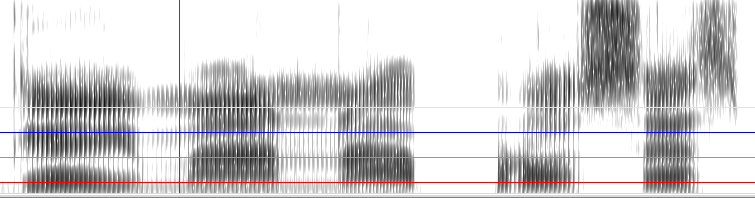
\includegraphics[width=0.95\linewidth]{images/target4.png}}
\subfigure[Generated speech]{
    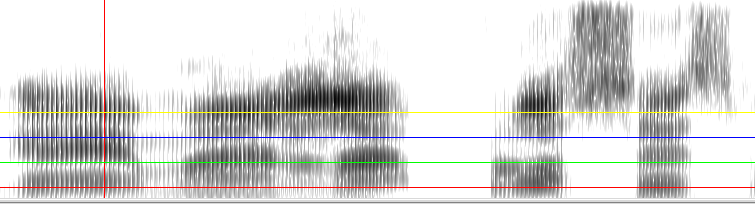
\includegraphics[width=0.95\linewidth]{images/generated4.png}}
\subfigure[Converted speech]{
    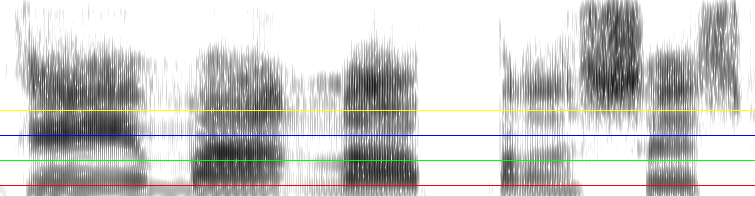
\includegraphics[width=0.95\linewidth]{images/transferred4.png}}
  \caption{Spectrograms of original, generated, and converted speech. The source speaker is female while the target speaker is male.\label{fig:waveform}}
\end{figure}


\subsection{VACONDA}

The architecture of our model is built on top of VQ-VAE. It consists of three modules: an encoder, quantizer and a decoder. As our encoder, we use a dilated convolution stack of layers which downsamples the input audio by 64. The speech signal was power normalized and squashed to the range (-1,1) before feeding to the downsampling encoder. To make the training faster, we have used chunks of 2000 time steps. This means we get 31 timesteps at the output of the encoder. The quantizer acts as a bottleneck and performs vector quantization to generate the appropriate code from a parameterized codebook. We define the latent space $e \in \mathbmm{R}^{k\times d}$ to contain $k$ $d$-dim continuous vector. Quantization is implemented using minimum distance in the embedding space. The number of classes was chosen to be 64, approximating 64 universal phonemes. We use a linear mapping to first project the 128 dimensional vector to 160 dimensions. We then perform comparisons with respect to individual articulatory dimensions each of which is 16 in size.  Assuming $z_e(x)$ denotes the encoder output in the latent space, then the input of decoder $z_d(x)$ will be obtained by $\argmin_{j}d(e_j, z_e(x))$, where $d$ is a similarity function of two vectors. In this paper, we consider Euclidean distance as the similarity metric.  Our decoder is an iterated dilated convolution-based WaveNet that uses a 256-level quantized raw signal as the input and the output from vector quantization module as the conditioning. Although using a Mixture of Logistics loss function might yield a better output, we have only used a 256 class softmax in this study. The decoder takes the output from the quantizer along with the speaker label as global conditioning and aims to reconstruct the input in an autoregressive fashion. Following IDCNNs, we have shared the parameters of all the stacks.



% In this subsection we describe our end-to-end approach for the task. We extend the framework proposed in \citep{vq-vae} to accomplish subword unit discovery. Although a structure such as HMM \citep{hmm-vae_bhiksha} might be intuitively better at capturing the transitions, we have limited ourselves to a vector quantization based approach as we observed it to be better at handling the posterior collapse problem in VAEs. We have used 3 stacks of 10 layers each in the decoder and residual blocks with similar dilation factors in each of the stacks shared their parameters \citep{strubell2017fast}.

% Our voice building process employs the VQ-VAE approach as outlined in \citep{rallabandi_mixedlingual_IS2017}, where the raw audio is first fed to a downsampling encoder which reduces the time resolution by 64. This encoded representation is then hashed into a latent representation that is forced to follow articulatory constraints. Specifically, we employ a set of discrete embeddings of cardinality 5, where each is a multi-dimensional array in itself associated with a continuous vector. The output from this hash function is fed to the decoder, which is a conditional WaveNet implemented using iterated dilated convolutions. In this section, we first present our analysis of the optimization that happens in our models. We then present a case for controlling the disentanglement that happens in such models to accomplish voice conversion. This is followed by an explanation of each component in our model in detail.

% Aside from the architecture discussed in Section~\ref{proposed_approach}, we argue that adding meaningful inductive bias can help the model learn better. We first normalize the vector representation to ensure the same scale in the latent space. Compared to VQ-VAE, we incorporate the articulatory features information in Table~\ref{tab:arti}. The above articulatory features apply to all human languages. To incorporate them, we first transpose the embedding from 128-dimension to 160-dimension by a linear layer. Then, we equally divide the latent embedding into 10 parts, and perform the vector quantization separately. Finally we concatenate all vectors, and feed into the linear layer to map it back to 128-dimension. In each class, the number of latent embedding is the number of possible values.


\subsection{Analysis}

In this section, we will discuss different design choices in the architecture, including input features and latent space constraints. 

% \subsubsection{Input Feature}

% We first compare the performance gap between different features as our model's input. The feature used along with its performance is shown in Table~\ref{tab:input}.

\subsubsection{Acoustic Unit Discovery}

Here we analyze the AUD performance of three different models in ZeroSpeech dataset as shown in Table~\ref{tab:aud}. We only show the results in English since we don't have ground truth for the Indonesian language.

% Now all is baseline 

\renewcommand{\arraystretch}{1.1}
\begin{table}[!htbp]
\caption{Performance of different systems in ZeroSpeech}
\centering
\begin{tabular}{l c c}\toprule[\heavyrulewidth]
& \multicolumn{2}{c}{English}\\
Model & ABX score & bitrate \\
\toprule[\heavyrulewidth]
Baseline & \textbf{27.46} & 74.5\\
Three-stage Model & 34.86 & 68.54 \\
VACONDA & 38 & \textbf{58.19} \\

\bottomrule[\heavyrulewidth]
\end{tabular}
\label{tab:aud}
\end{table}

As in Table~\ref{tab:aud}, the VACONDA achieves the best bit rate among three models. With such small number of unit, we could resynthesize and even convert the speech in a very high quality.

\subsubsection{Speech Resynthesis and Conversion}

The proposed model supports synthesizing the same speech in both the same speaker and a different speaker. Here we show a sample in the test dataset of Indonesian language in Figure~\ref{fig:waveform}. When we feed the decoder with the same speaker identification, the decoder will generate the original audio. Otherwise, it will perform speech convertion. The three audio shares similar structure.  However, the converted audio has denser waveform, suggesting it's a different speaker. For the sampled audio, please visit the \href{http://tts.speech.cs.cmu.edu/rsk/campaigns/interspeech2019/submissions/acoustic_unit_discovery/}{our website}.



%The results are shown in Table~\ref{tab:constraints}. We use 

% \renewcommand{\arraystretch}{1.1}
% \begin{table}[htbp]
% \caption{System performance with latent space constraints}
% \centering
% \begin{tabular}{l | c}\toprule[\heavyrulewidth] \textbf{Model} & \textbf{ABX score}\\
% \toprule[\heavyrulewidth]
% Baseline model & 12\\
% \bottomrule[\heavyrulewidth]
% \end{tabular}
% \label{tab:constraints}
% \end{table}

\label{analysis}


\subsection{Conclusion}

In this case study, we present an approach to automatically discover acoustic-phonetic units from a speech utterance in an unsupervised fashion. We first present an analysis to show that incorporating latent random variables into neural generative models using suitable priors allows us to control what gets encoded into the latent space. Based on this, we employ articulatory features as a discrete prior bank in the latent space and obtain acoustic units that are speaker and language independent.  To validate effectiveness of the discovered units, we perform discriminability tests as part of ZeroSpeech Challenge 2019. 


\section{De-Entanglement of Content - Application to Source Separation}



\noindent Speech synthesis has taken some major strides in past few years especially in the form of text-2-speech synthesis (TTS) models. However, most of the work that has been carried out involves carefully recorded speech data. Generation of such vast amount of data for every application is a daunting task. On the other hand, there is a plethora of speech data that is available on the internet such as news broadcasts, press conferences, audio books etc - also referred to as \textit{Found Data}. The only hindrance in utilizing such data for speech based machine learning models is that this found data is characterized by noise or music in the background. Presence of noise / music degrades the performance of such models. One of the solutions to this problem is source separation - separating out speech from music in the audio. There have been several attempts to accomplish this task using both classical speech processing techniques as well as deep learning models.\\

\cite{6287816} proposed a matrix factorization of the magnitude spectrogram of audio that utilizes the periodicity in music and sparseness in speech to separate the two. However, this technique requires a lot of hyperparameter tuning depending on the type of background music and also degrades the quality of separated speech to some extent. REPET \cite{6269059} also involves music separation by exploiting its periodic nature but on occasions still leaves a residual music in the background. Most of the work in source separation using deep learning has been supervised \cite{SVSGAN}, \cite{Disc}, \cite{TFGAN}, \cite{spen}, i.e. they had both noisy and clean versions of the data. However most of the times, especially with found data, we don't have the clean version of the data. \\

There has also been some focus on source separation using unsupervised models. \cite{Hsu2018DisentanglingCS} takes the approach of data augmentation by adding different background noise to the clean data and then training an adversarial classifier to make these augmented versions of data indistinguishable from the original speech. However, this method again requires a clean version of data first and additional data augmentation that is representative of the noise in the background. Therefore essentially, this is a semi-supervised approach that requires labels for clean and noisy data. One other semi-supervised approach is using domain adaptation \cite{domadp} where output is made to follow the clean data domain while making the encoding for clean and noisy data domain indistinguishable using a adversarial classifier. However, this approach requires speech content in both clean and noisy version of data to be very similar for domain adaptation to occur. \\

We propose a completely unsupervised approach using multinode variational autoencoders (VAE) combined with robust principal component analysis (RPCA) \cite{6287816} as a post-processing step. Our goal is to enable the use of found data for downstream TTS applications. Therefore, the data we target is predominantly speech with music in the background. We apply this approach on two datasets:- Wilderness\cite{wildernessdataset} and Hub4. Wilderness consists of Bible recordings in 699 languages while Hub4 is a news broadcast dataset in English. Both of these datasets contain music/noise in the background. We show that the proposed approach separates out the dominant mode, speech, from a noisy audio and improves the performance of the downstream tasks irrespective of the language of the speech. \\

This paper is organized as follows: section 1 discusses the variational autoencoder framework, section 2 talks about source separation using VAE, section 3 addresses the extension to multinode VAE architeture and section 4 discusses post-processing using robust principal component analysis (RPCA). Section 5 analyses the source separation capacity and architectural requirements of the proposed model. Section 6 reports the performance of the proposed model for source separation and for downstream TTS applications. We conclude in section 7.

\section{Variational Autoencoder}
Variational autoencoder model in this paper follows the standard formulation consisting of an inference network with a speech encoder $p(z|x)$ and a latent space decoder $p(x|z)$, where $x$ and $z$ represent the input and the latent space random variables respectively. 

\begin{figure}[h!]
    \centering
    \includegraphics[scale=0.4]{LatexDiss/Dissertation/images/vae_graph.png}
    \caption{Latent Variable Model - Variational Autoencoder}
    \label{fig:vae_graph}
\end{figure}


The figure \ref{fig:vae_graph} depicts the latent variable model for variational autoencoder. The true posterior density is intractable.

\begin{equation}
    p(z|x) = \frac{p(x|z)p(z)}{p(x)}
\end{equation}
% Intractable true posterior and marginals
% ELBO formulation


We then approximate the true posterior $p(z|x)$ with a variational distribution $q(z|x)$ that has a prior $p(z)$. The objective can be represented by the evidence lower bound (ELBO) or variational lower bound on the likelihood of the data. 
\begin{equation}
    \log{p(x)} \geq \mathcal{L}(x)
\end{equation}

\begin{equation}
\mathcal{L}(x) = \mathbb{E}_q[\log(p(x|z))] - D_{KL}(q(z|x) || p(z)) 
\label{Likelihood}
\end{equation}

where $\mathcal{L}(x)$ denotes the variational lower bound on the likelihood of the data and $D_{KL}$ is the Kullback-Leibler divergence. We write the first term as a mean squared error (MSE) between the reconstructed and the original data and the prior p(z) follows a standard normal distribution $\mathcal{N}(0,I)$.

\section{VAE for Source Separation}
As shown in the previous section, a variational autoencoder reconstructs the input data conditioned on the latent space. The latent space is constrained to follow a certain prior distribution, such as Gaussian distribution. \cite{JMLR:v19:17-704} shows that this formulation is equivalent to minimizing the alternative lower bound function 

\begin{equation}
\begin{aligned}
minimize \;\; & n \cdot rank[\, L \,] \,+ \parallel S \parallel_0   \\
M & = L + S \\
\end{aligned}
\end{equation}


where M is the original data matrix, L is a low-rank matrix and S is a sparse matrix and $\parallel.\parallel_0$ denotes the $l_0$ norm. This is shown to be equivalent to an RPCA problem if an optimum solution exists otherwise it's known to smooth out undesirable erratic peaks from the energy curve. \cite{JMLR:v19:17-704} also presents some interesting results on VAE and it's separation properties. We rewrite some of the results what it means in our context here.


\begin{itemize}
    \item This formulation of variational autoencoders is shown to perform robust outlier removal in the context of learning inlier points constrained to a manifold of unknown dimension. In simple terms this means, VAE has the property to remove sparse components in the input data distribution and accordingly reduces the latent space to a required (unknown) dimension.
    \item VAE also help smooth out undesirable minima from the energy landscape of the optimization problem which differentiates it from traditional deterministic autoencoders.
\end{itemize}
 
Since our goal is to enhance speech synthesis and speech recognition performances on the 'found' data, we target audio data that is predominantly speech with some music (almost uniform) in the background, for instance, news broadcasts and audio books. We will later show that the presence of the background music can effect the speech synthesis performance drastically. It's been shown that speech and music distributions in audio are quite distinct \cite{SM_diff} \cite{SM_diff1}. As a result VAE has the tendency to remove the sparse outlier - music from the audio. \\ 

In case of multiple speakers in the input audio there can be multiple modes in the speech distribution as well. This can be solved by have multiple nodes in the latent space. This is possible because all latent variables are initialized at random and pick multiple speech modes from the distribution. Later in the results section, we are going to analyze this and the requirement on the number of nodes in the latent space depending on the input data distribution. We also talk about how the performance of the output speech changes based on the intensity/loudness of the music in the background.

\section{Multi-node VAE Model Architecture}


\begin{figure}
    \centering
    \includegraphics[scale=0.31]{LatexDiss/Dissertation/images/Multinode_VAE.jpg}
    \caption{Multi-node VAE model. Dashed lines represent sampling using reparametrization. Encoder and Decoder are Bi-LSTM networks. Purple blocks are fully connected layers.}
    \label{fig:VAE}
\end{figure}

The Figure \ref{fig:VAE} depicts the multi-node variational autoencoder architecture. It consists of an Bi-LSTM encoder ($LSTM_E$) for the inference network that captures latent space distributions $p(z_1|x), p(z_2|x), \dots, p(z_k|x)$ where $x$ is the magnitude spectrogram of the input audio, $z_1, z_2, \dots, z_k$ are the latent variables and $k$ is the number of latent variables. The reconstruction network is a Bi-LSTM decoder ($LSTM_D$) which generates the reconstructed input distribution at each time-step $p(x_r^t|x_r^{t-1},z_1,z_2,\dots,z_k)$ conditioned on the reconstructed input from the previous time-step and the latent space. 

\begin{equation}
h_e^t, c_e^t = LSTM_E(x^t,h_e^{t-1},c_e^{t-1})
\end{equation}
\begin{equation}
\mu_i^t = MLP_{\mu_i}(h_e^t) \; \forall i \in {0,\dots,k}
\end{equation}
\begin{equation}
logvar_i^t = MLP_{\sigma_i}(h_e^t) \; \forall i \in {0,\dots,k}
\end{equation}
\begin{equation}
q(z_i|x) = \mathcal{N}(\mu_i,\exp(logvar_i))
\end{equation}
\begin{equation}
h_{d}^t, c_{d}^t = LSTM_D(\phi^t, z_1^t, \dots, z_k^t,h_d^{t-1},c_d^{t-1})
\end{equation}
\begin{equation}
\phi^t = MLP_{\phi}(h_d^{t-1})
\end{equation}
\begin{equation}
x_r^t = MLP_{x_r}(h_d^t)
\end{equation}

where Bi-LSTM refers to bidirectional long short term memory recurrent neural network, MLP refers to a multi-layer perceptron network, $h_e, c_e$ represent hidden and cell states of the encoder LSTM, $h_d, c_d$ represent hidden and cell states of the decoder LSTM and $\phi$ represents the context from the previous time-step of the decoder. The initial hidden state and the cell state of the decoder LSTM are learnable parameters. The latent variable model for the multinode variational autoencoder is shown in figure \ref{fig:multinodevae_graph}\\

\begin{figure}[h!]
    \centering
    \includegraphics[scale=0.4]{LatexDiss/Dissertation/images/multinode_vae_graph.png}
    \caption{Latent Variable Model - Multinode Variational Autoencoder}
    \label{fig:multinodevae_graph}
\end{figure}

The modified learning objective for a multinode VAE can be represented as an extension of equation \ref{Likelihood} as:

\begin{equation}
\begin{aligned}
\mathcal{L}(x) \ge & \; \mathbb{E}_q[\log(p(x|z_1,z_2,\dots,z_k))] \\& -\sum_{i=1}^k D_{KL}(q(z_i|x) || p(z_i)) 
\end{aligned}
\end{equation}



\section{Speech Enhancement}

The output of the VAE network from the above formulation removes the music from the audio however, replaces the music content with random noise instead of silence. There can be multiple post processing or speech enhancement techniques used to eliminate this residual noise such as speech enhancement neural networks or classical speech processing methods. Here in this paper we use robust principal component analysis (RPCA) \cite{6287816} to eliminate the background noise as it gives control over the quality of speech versus the amount of background noise. We follow the original formulation from the paper by expressing the speech separation as a matrix factorization problem. It represents the magnitude spectrogram of the audio signal as a sum of low rank matrix and a sparse matrix. The assumption here is that non-speech component (background noise) is low rank while the speech component is sparse. 

\begin{equation}
\begin{aligned}
minimize & \parallel L \parallel_* + \lambda \parallel S \parallel_1   \\
M & = L + S
\end{aligned}
\end{equation}

where $M \in \mathbb{R}^{n_1 \times n_2}$ is the magnitude spectrogram of the VAE output, $L \in \mathbb{R}^{n_1 \times n_2}$ is a low rank matrix, $S \in \mathbb{R}^{n_1 \times n_2}$ is a sparse matrix, $\parallel . \parallel_*$ is the nuclear norm and $\parallel . \parallel_1$ is the $L_1$ norm. $\lambda > 0$ is a hyperparameter that controls the rank and sparsity of $L$ and $S$ respectively. It is recommended in \cite{6287816} to use $\lambda = 1/\sqrt{max(n_1,n_2)}$ to obtain the best result. However, we only need to enhance the audio a little while retaining the speech quality so we use $\lambda = 0.3/\sqrt{max(n_1,n_2)}$. Instead of the hard mask in \cite{6287816} we used a soft mask as it resulted in a better quality and a smoother speech. The idea is to have a high value for the speech mask where the magnitude of the speech component is much greater the magnitude of the non-speech component.

\begin{equation}
|S|  > g|L|
\end{equation}

\begin{equation}
|S|^2  > g^2 |L|^2
\end{equation}

\begin{equation}
|M|^2  = |S|^2 + |L|^2
\end{equation}

\begin{equation}
|S|^2  > g^2 |M|^2 - g^2|S|^2
\end{equation}

\begin{equation}
|S|^2  > \frac{g^2}{1 + g^2} |M|^2 
\end{equation}

\begin{equation}
|S|  > \sqrt{\frac{g^2}{1 + g^2}} |M|
\end{equation}

\begin{equation}
\frac{|S|}{|M|} - \sqrt{\frac{g^2}{1 + g^2}} > 0 
\end{equation}

where $g \ge 0$ is the gain factor. We came up with a Sigmoid looking threshold for the mask which is still close to the hard mask but results in smoother speech transitions.  

\begin{equation}
W = \frac{1}{1 + \exp{(-\alpha(\frac{|S|}{|M|} - \sqrt{\frac{g^2}{1 + g^2}}))}}
\end{equation}

where $W \in \mathbb{R}^{n_1 \times n_2}$ represents the speech mask and the obtained speech spectrogram is

\begin{equation}
X_{speech}(i,j) = W(i,j)M(i,j) \; \forall i,j
\end{equation}

\section{Experiments}
We applied the multinode VAE model on two datasets:- Wilderness and Hub4. Wilderness dataset consists of Bible recordings in 699 languages with music in the background. We carried out full experiments on two languages:- Dhopadhola (an African language) and Marathi (an Indian language). The results presented here are based on the model that was trained on languages different than the ones that are reported/tested. Hub4 consists of news broadcast recordings in English with various forms of noise in the background, such as music, clapping, roaring etc. We used about 2 hrs of training data for both datasets consisting 1 hr of speech only data and 1 hr of speech-music data. \\

For these experiments, the VAE model consists of input magnitude spectrogram of dimension 512, Bi-LSTM encoder and decoder with hidden size of 512, each of the fully connected layers for latent variables and decoder context from the previous time-step of dimension 64 and the final output layer with a dimension same as the input dimension. We trained for 50 epochs with annealing weight for KL-Divergence loss, this is explained in detail below. For both datasets, we used an ADAM optimizer with a learning rate of 1e-3. \\ 


\begin{figure}[h!]
    \centering
    \begin{subfigure}{0.2\textwidth}
    \includegraphics[scale=0.55]{LatexDiss/Dissertation/images/wilderness_hist.png}
    \caption{Wilderness}
    \end{subfigure}
    \hspace*{\fill}
    \begin{subfigure}{0.2\textwidth}
    \includegraphics[scale=0.55]{LatexDiss/Dissertation/images/hub4_hist.png}
    \caption{Hub4}
    \end{subfigure}
    \caption{Input Data Distributions for (a) Wilderness (b) Hub4. The red dots show the high density regions in each distribution.}
    \label{fig:distributions}
\end{figure}

The input data distributions for the two dataset are shown in Figure \ref{fig:distributions}. These 2-dimensional distributions are obtained after applying PCA to the magnitude spectrogram and plotting the histogram of the first two components. This figure shows the high density regions of the two distributions. As we can observe, the wilderness distribution has one significant high density region while the hub4 distribution consists of multiple high density regions. Hence, Hub4 data will have more dominant speech modes than the wilderness data. This is probably because there are multiple speakers in Hub4 as well as news broadcast speech has more variance as compared to bible recordings. This gives us an approximate idea that Hub4 multinode VAE model will require more nodes in the latent space than the model for Wilderness dataset. \\

\begin{figure}[h!]
    \centering
    \includegraphics[scale=0.37]{LatexDiss/Dissertation/images/score1.png}
    \caption{Gaussian Mixture Fit for Wilderness and Hub4}
    \label{fig:GMM}
\end{figure}

Figure \ref{fig:GMM} shows the likelihood of fitting Gaussian Mixture Models as a function of the number of cluster centers. As discussed earlier, speech modes are dominant in the target data so fitting $n$ clusters in the curve can be thought of as having $n-1$ nodes/clusters in the VAE for the speech and $1$ cluster as the residual non-speech data. The multinode VAE model for the wilderness data obtained good results with just $1$ VAE node or $2$ clusters as can be confirmed from the graph where likelihood values are high for just $2$ clusters. On the other hand, multinode VAE model for Hub4 gave good results with $3$ nodes or $4$ clusters. Now, as we increase the number of nodes, the peak performance does not change much, however, we attain the same peak performance for more model states:- MSE loss vs KL loss. This will be explained using training loss curves. It would have been better to use some validation parameter but since model performance for human hearing can only be analyzed by listening to the speech, we use the training metrics. \\


\begin{figure}[h!]
    %\centering
    \begin{subfigure}{0.4\textwidth}
    \centering
    \includegraphics[scale=0.31]{LatexDiss/Dissertation/images/unsupervised1_w.png}
    \caption{1-Node VAE: Wilderness}
    \end{subfigure}
    \vspace{0pt} \newline
    \begin{subfigure}{0.4\textwidth}
    \centering
    \includegraphics[scale=0.31]{LatexDiss/Dissertation/images/unsupervised3_w.png}
    \caption{3-Node VAE: Wilderness}
    \end{subfigure}
    \caption{Training Loss (a) 1-Node VAE: Wilderness (b) 3-Node VAE: Wilderness. The left shaded blue region and the right shaded orange region show the required MSE loss and KL loss threshold respectively to obtain good speech. Overlap region represents the model parameters where speech separation occurs.}
    \label{fig:lossw}
\end{figure}




The Figure \ref{fig:lossw} and \ref{fig:lossh} give an idea of speech separation capacity of the model as we increase the number of latent variables. During training of the multinode VAE model, we anneal the KL divergence loss for latent space exponentially. We do the annealing for latent variables simultaneously. Initially, KL divergence loss is assigned a very small weight and then increased exponentially. So, it first increases (not shown in the plot as it's out of the range of the plot) and then decreases eventually while the MSE reconstruction loss first decreases and then increases slightly. During this process there is a small window where both the losses are low enough and we are able to extract out speech from the audio. This window is determined by the threshold values for both losses. If both loss values are below their respective thresholds, we observe speech at the output.\\


\begin{figure}[h!]
    %\centering
    \begin{subfigure}{0.4\textwidth}
    \centering
    \includegraphics[scale=0.31]{LatexDiss/Dissertation/images/unsupervised1_h.png}
    \caption{1-Node VAE: Hub4}
    \end{subfigure}
    \vspace{0pt} \newline
    \begin{subfigure}{0.4\textwidth}
    \centering
    \includegraphics[scale=0.31]{LatexDiss/Dissertation/images/unsupervised3_h.png}
    \caption{3-Node VAE: Hub4}
    \end{subfigure}
    \vspace{0pt} \newline
    \begin{subfigure}{0.4\textwidth}
    \centering
    \includegraphics[scale=0.31]{LatexDiss/Dissertation/images/unsupervised8_h.png}
    \caption{8-Node VAE: Hub4}
    \end{subfigure}
    \caption{Training Loss (a) 1-Node VAE: Hub4  (b) 3-Node VAE: Hub4 (c) 8-Node VAE: Hub4. The left shaded blue region and the right shaded orange region show the required MSE loss and KL loss threshold respectively to obtain good speech. Overlap region represents the model parameters where speech separation occurs.}
    \label{fig:lossh}
\end{figure}

The blue and orange shaded regions in figures \ref{fig:lossw} and \ref{fig:lossh} depict the loss values below the threshold for MSE loss and KL divergence loss respectively. Therefore, their intersection as indicated by the overlap region represents the model parameters that result in speech and music separation. For visualization, the MSE loss in the figure is averaged over all the samples as well as in the time dimension of the audio while the KL divergence loss is averaged over all the latent variables as well as across all samples. Using these loss definitions results in a threshold value of 250 for MSE loss and a threshold value of 60 for KL divergence loss for both datasets. These are just soft experimental values and may change for other datasets as well as a different loss definition. The key idea is that there exists a window where speech separation occurs. \\



As shown in the figure, for Wilderness data we obtain this window with just one node in the latent space. As we increase the number of nodes in the latent space, we don't see any significant improvement in the quality of the output speech, however, we do obtain a wider window where this separation occurs. As for the Hub4 dataset, we don't observe any such window with one latent node, however, we do obtain a separation window with three latent nodes and an even wider window with eight latent nodes. Observe that, these results align with the results derived using input data distribution and GMM fitting analysis. Therefore, to be totally certain about the existence of a separation window, we can always add a few more latent variables than what we obtain from our analysis of input distribution. \\

Let's explore the nature of the output on either side of the separation window. On the blue/left side of the window MSE loss is very low while the KL divergence loss is high, this results in the output that is close to the original input that consists of both speech and music. On the orange/right side of the window, MSE loss is high while the KL divergence loss is low. This causes the network output to be a really noisy version of the speech component of the audio.  \\

We also observed that, as the intensity/loudness of music in the background increases in an audio or for a part of the audio, the speech separation performance for that part of the audio begins to deteriorate slightly. For example, in case of advertisement segments between news broadcasts where music tends to dominate the segment. In such cases, we can still hear some traces of music in the background when we use the same VAE model as we do for the rest of the data. However, this is not a concern as the downstream applications we target don't generally depend on data with such high intensity music. \\

As mentioned in \cite{JMLR:v19:17-704}, a traditional autoencoder is not able to perform the outlier removal. We verified this fact experimentally. We removed any constraint on the latent space and trained the model to minimize the reconstruction loss. We observed that the model was able to reconstruct the audio completely including both speech and music. Therefore, a traditional autoencoder is not able to smooth out the energy contour and fails to remove any outliers. We also tried to experiment with this model on songs and movie clips. As the background music in songs and movies very dense and varies significantly, we observed that our model wasn't able to separate out speech completely. The output speech contained some music in the background and the quality of speech itself was compromised.  

% Songs
% TV shows/ Movies

\section{Results}
%The separated speech samples for both Wilderness and Hub4 datasets can be found in the supplemental material
The separated speech samples for both Wilderness and Hub4 datasets can be found at \footnote[1]{https://github.com/nishantgurunath/Separabl/tree/master/samples}
under folders "Wilderness" and "Hub4" respectively. We present Wilderness samples for two languages - Dhopadhola and Marathi both having different but somewhat uniform music in the background. These samples can be found inside their respective folders within the wilderness folder. We also present samples for when we removed the KL-divergence term from the loss function and trained an autoencoder instead. It can be observed from the samples that the model reconstructs the whole audio without outlier/music removal. Hub4 data samples have a lot more variation in both speech and music. All the samples come from news broadcast in English. We also ran experiments on mixed signals where a background music was added to a clean sample from the wilderness data. We performed this experiment with drums, flute, guitar and piano music in the background. 
%The mixed audio and the separated speech samples can be found in the supplemental material.\\ 
The mixed audio and the separated speech samples can be found at \textsuperscript{\rm 1}.\\ 
% Do on some standard dataset
\begin{table}[h!]
    \centering
    \begin{tabular}{|c|c|c|}
    \hline
     \textbf{Input Audio} & \textbf{SegSNR} & \textbf{MOS} \\
     \hline
     Noisy &  4.91 & 1.5 \\
     \hline
     Clean & 7.5 & 1.2\\
     \hline
    \end{tabular}
    \caption{Segmented Signal to Noise Ratio (SegSNR) and Mean Opinion Score (MOS) for Mixed Signals}
    \label{tab:my_label}
\end{table}

\begin{table}[h!]
    \centering
    \begin{tabular}{|c|c|c|}
    \hline
     \textbf{Audio} & \textbf{WER Mono Voxforge} &  \textbf{WER Tri2b Librispeech}\\
     \hline
     Noisy &  100.53 & 103.72 \\
     \hline
     Clean & 102.84 &  104.33 \\
     \hline
    \end{tabular}
    \caption{Word Error Rate (WER) for Noisy and Cleaned Audio on Pretrained Kaldi ASR Models}
    \label{tab:my_label}
\end{table}

One other way to asses the proficiency of the proposed method is to evaluate its performance on downstream tasks, for instance, Text-2-Speech Synthesis (TTS). We performed Text-2-Speech synthesis on original and cleaned version of Marathi language from the wilderness dataset. 
%The TTS samples can be found with the supplemental material as well. 
The TTS samples can be found at \textsuperscript{\rm 1} as well.
We observe that Text-2-Speech synthesis performance improves significantly after music is removed from the background. In TTS samples generated from the original (noisy) version of the audio, one can clearly see the distortion in the speech and presence of music in the background. Whereas, TTS samples that were generated from cleaned samples had a very clear speech quality with no music in the background. 




% TTS with noisy - speech breaks and music in the background

\section{Conclusion}
We show that Multinode VAE model helps to remove the background noise/music in the 'found data' irrespective of the language of the speech. Extensive studies on different type of speech and music data verify the effectiveness and robustness of the proposed approach. Performance of this model on Text-2-Speech synthesis applications shows the potential of such an approach that can be further extended to other speech based machine learning models such as Automatic Speech Recognition (ASR). Such an efficient source separation technique can help overcome a major cause for under utilization of 'found data'. This could mean that acoustic based machine learning models can be drastically improved by leveraging the data found on the internet. Since this approach works in a unsupervised fashion, it eliminates the need to obtain labeled data which has been major hindrance to effective utilization of 'found data'. Since 'found data' is abundant, this could also possibly further accelerate the research in this area. 

